\documentclass{beamer}

\mode<presentation>{
	%\usetheme{CambridgeUS}
	%\usecolortheme{seahorse}
	\usetheme{Boadilla}
	\usecolortheme{beaver}
	\setbeamertemplate{navigation symbols}{}
}

\usepackage{graphicx}
\usepackage{booktabs}
\usepackage{algpseudocode}
\usepackage{hyperref}
\usepackage{tikz}
\usepackage[utf8]{inputenc}
\usepackage{listings}
\usepackage[export]{adjustbox}
\usepackage{aeguill}

%\setbeamertemplate{title page}[default][rounded=false]

\setbeamertemplate{title page}
{
%\vbox{}
\begingroup
\centering
\begin{beamercolorbox}[sep=8pt,center]{institute}
\usebeamerfont{institute}\insertinstitute
\end{beamercolorbox}
\vskip1em%
\begin{beamercolorbox}[sep=8pt,center]{title}
\usebeamerfont{title}\inserttitle\par%
\ifx\insertsubtitle\@empty%
\else%
\vskip0.25em%
{\usebeamerfont{subtitle}\usebeamercolor[fg]{subtitle}\insertsubtitle\par}%
\fi%
\end{beamercolorbox}%
\vfill
\begin{beamercolorbox}[sep=8pt,center]{author}
\usebeamerfont{author}\insertauthor
\end{beamercolorbox}
\vskip1em\par
\begin{beamercolorbox}[sep=8pt,center]{date}
\usebeamerfont{date}\insertdate
\end{beamercolorbox}
\endgroup
}

\setbeamertemplate{blocks}[default]
\setbeamercolor{structure}{fg=darkred}
%\setbeamercolor{block title}{bg=darkred,fg=white}
%\setbeamercolor{block body}{bg=darkgray!20!white}
\setbeamercolor{block title}{bg=darkgray!30!white}
\setbeamertemplate{enumerate items}[default]

\setbeamertemplate{part page}{
\begin{beamercolorbox}[sep=8pt,center,wd=\textwidth]{part title}
\usebeamerfont{part title}\insertpart\par
\end{beamercolorbox}
\vfill
\tableofcontents
}

%\setbeamertemplate{frametitle continuation}{(\insertcontinuationcount)}

\setbeamertemplate{headline}{\leavevmode\hbox{\begin{beamercolorbox}[wd=.5\paperwidth,ht=2.65ex,dp=1.5ex,center]{section in head/foot}\usebeamerfont{section in head/foot}\insertsectionhead\hspace*{2ex}
\end{beamercolorbox}\begin{beamercolorbox}[wd=.5\paperwidth,ht=2.65ex,dp=1.5ex,center]{subsection in head/foot}\usebeamerfont{subsection in head/foot}\hspace*{2ex}\insertsubsectionhead\end{beamercolorbox}}\vskip0pt}

\setbeamertemplate{background}{\tikz[overlay,remember picture]\node[opacity=0.08]at (current page.south east){
\includegraphics[width=10cm]{figures/unibo_logo.jpg}};}

\newcommand{\tcc}[1]{\textcolor{darkred}{#1}}

\newcommand{\codeA}[1]{\texttt{#1}}
\newcommand{\codeB}[1]{\texttt{\textcolor{darkred}{#1}}}

\newcommand{\link}[1]{{\footnotesize » \url{#1}}}
\newcommand{\bothquote}[1]{``#1''}

\definecolor{mygreen}{rgb}{0,0.6,0}
\definecolor{mygray}{rgb}{0.5,0.5,0.5}
\definecolor{mymauve}{rgb}{0.58,0,0.82}
\definecolor{maroon}{rgb}{0.5,0,0}
\definecolor{darkgreen}{rgb}{0,0.5,0}

\lstset{
language=Java,
basicstyle=\scriptsize\ttfamily,
keywordstyle=\scriptsize\color{blue}\ttfamily,
commentstyle=\scriptsize\color{mygreen}\ttfamily,
breakatwhitespace=false,
breaklines=true,
 numbers=left,
  numberstyle=\color{mymauve},
  stringstyle=\color{mymauve},
  showstringspaces=false,
  numbers=none
}

\lstdefinelanguage{XML}
{
  basicstyle=\scriptsize\ttfamily,
  morestring=[s]{"}{"},
  morecomment=[s]{?}{?},
  morecomment=[s]{!--}{--},
  commentstyle=\color{darkgreen},
  moredelim=[s][\color{black}]{>}{<},
  moredelim=[s][\color{red}]{\ }{=},
  stringstyle=\color{blue},
  identifierstyle=\color{maroon},
  numbers=none
}

\makeatother

\AtBeginSection[]
{
  \begin{frame}
    \frametitle{Outline}
    \tableofcontents[currentsection]
  \end{frame}
}

%\AtBeginSubsection[]
%{
%  \begin{frame}
%    \frametitle{Outline}
%    \tableofcontents[currentsection,currentsubsection]
%  \end{frame}
%}

\institute[UNIBO]{\uppercase{Alma Mater Studiorum -- Università di Bologna}\\Dipartimento di Informatica -- Scienza e Ingegneria (DISI)\\C.d.S. in Ingegneria e Scienze Informatiche, Campus di Cesena}

\author[A. Marfoglia]{Alberto Marfoglia\\\scriptsize\texttt{alberto.marfoglia2@unibo.it}}


\title[Android -- 1A -- Intro]{Android programming}
\subtitle{Intro and fundamentals}
\date[ver. 1.0 (20220505)]{Embedded Systems and Internet of Things\\A.A. 2021 -- 2022}

\begin{document}

\begin{frame}
\titlepage 
\end{frame}

\newcommand\blfootnote[1]{%
  \begingroup
  \renewcommand\thefootnote{}\footnote{#1}%
  \addtocounter{footnote}{-1}%
  \endgroup
}

\begin{frame}{Thanks}
    \centering
    \begin{itemize}
      \item \large{Professor Angelo Croatti}
    \end{itemize}

    \blfootnote{\url{https://www.unibo.it/sitoweb/a.croatti/en}}
    \blfootnote{}
\end{frame}

\section{Intro}

\begin{frame}{Google Android}
\begin{block}{Overview}
Android is an operating system designed for use on mobile devices, based on Linux Kernel
\begin{itemize}
  \item Originally created for use in digital cameras
  \item Google acquired Android in 2005 for at least \$50 million (Google's \textit{"best deal ever"})
  \item Distributed under \textit{open-source} (Apache 2.0) license
\end{itemize}
\end{block}

\begin{block}{Embedded OS}
  Designed to run primarily on devices with a touch-screen interface.\newline
  Today, it's being used in:
  \begin{itemize}
    \item \tcc{Android TV}, \tcc{Android for Cars}, as well as \tcc{Android Wear devices}.
  \end{itemize}
\end{block}
\end{frame}

\subsection{Market Share}

\begin{frame}{Mobile OS Market Share}
  \begin{figure}
    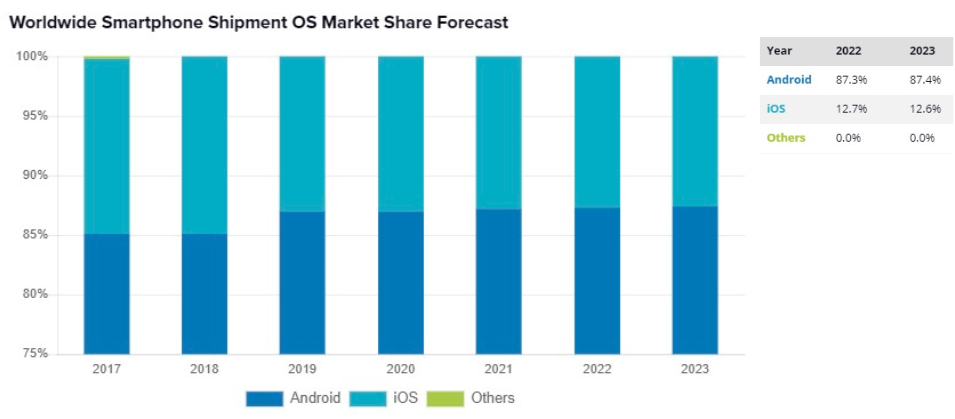
\includegraphics[width=1\linewidth]{figures/android-marketshare.png}
  \end{figure}
  \link{http://www.idc.com/prodserv/smartphone-os-market-share.jsp}
\end{frame}

\section{Android OS}

\begin{frame}{Android OS}
  \begin{block}{Based on Linux}
    \begin{itemize}
      \item Android is a Linux multi-user operating system (embedded).
      \item It's not a GNU/Linux distribution.
    \end{itemize}
  \end{block}
  \begin{block}{Security}
    Each Android app lives in its own security sandbox, protected by the following security features:
    \begin{itemize}
      \item Android OS is a multi-user Linux system (each app is a different user)
      \item Each app has its own virtual machine (isolation)
      \item The system assigns each app a unique ID with specific permissions
        \begin{itemize}
          \item \tcc{Least Privilege}
        \end{itemize}
      \item The permissions must be explicitly granted by the user 
    \end{itemize}
  \end{block}
\end{frame}

\begin{frame}{Android OS: Software Stack}
  \begin{columns}[c]
    \column{0.45\textwidth}
    \begin{itemize}\itemsep10pt
      \item \tcc{Java API Framework}: exposes the full feature-set over native libraries
      \item \tcc{ART}: application runtime environment
      \item \tcc {Native libraries}: \textit{C+/C++} code used to build many core components
      \item \tcc{HAL}: defines a standard interface for interacting with built in hardware component
    \end{itemize}
    \column{0.55\textwidth}
      \begin{figure}
       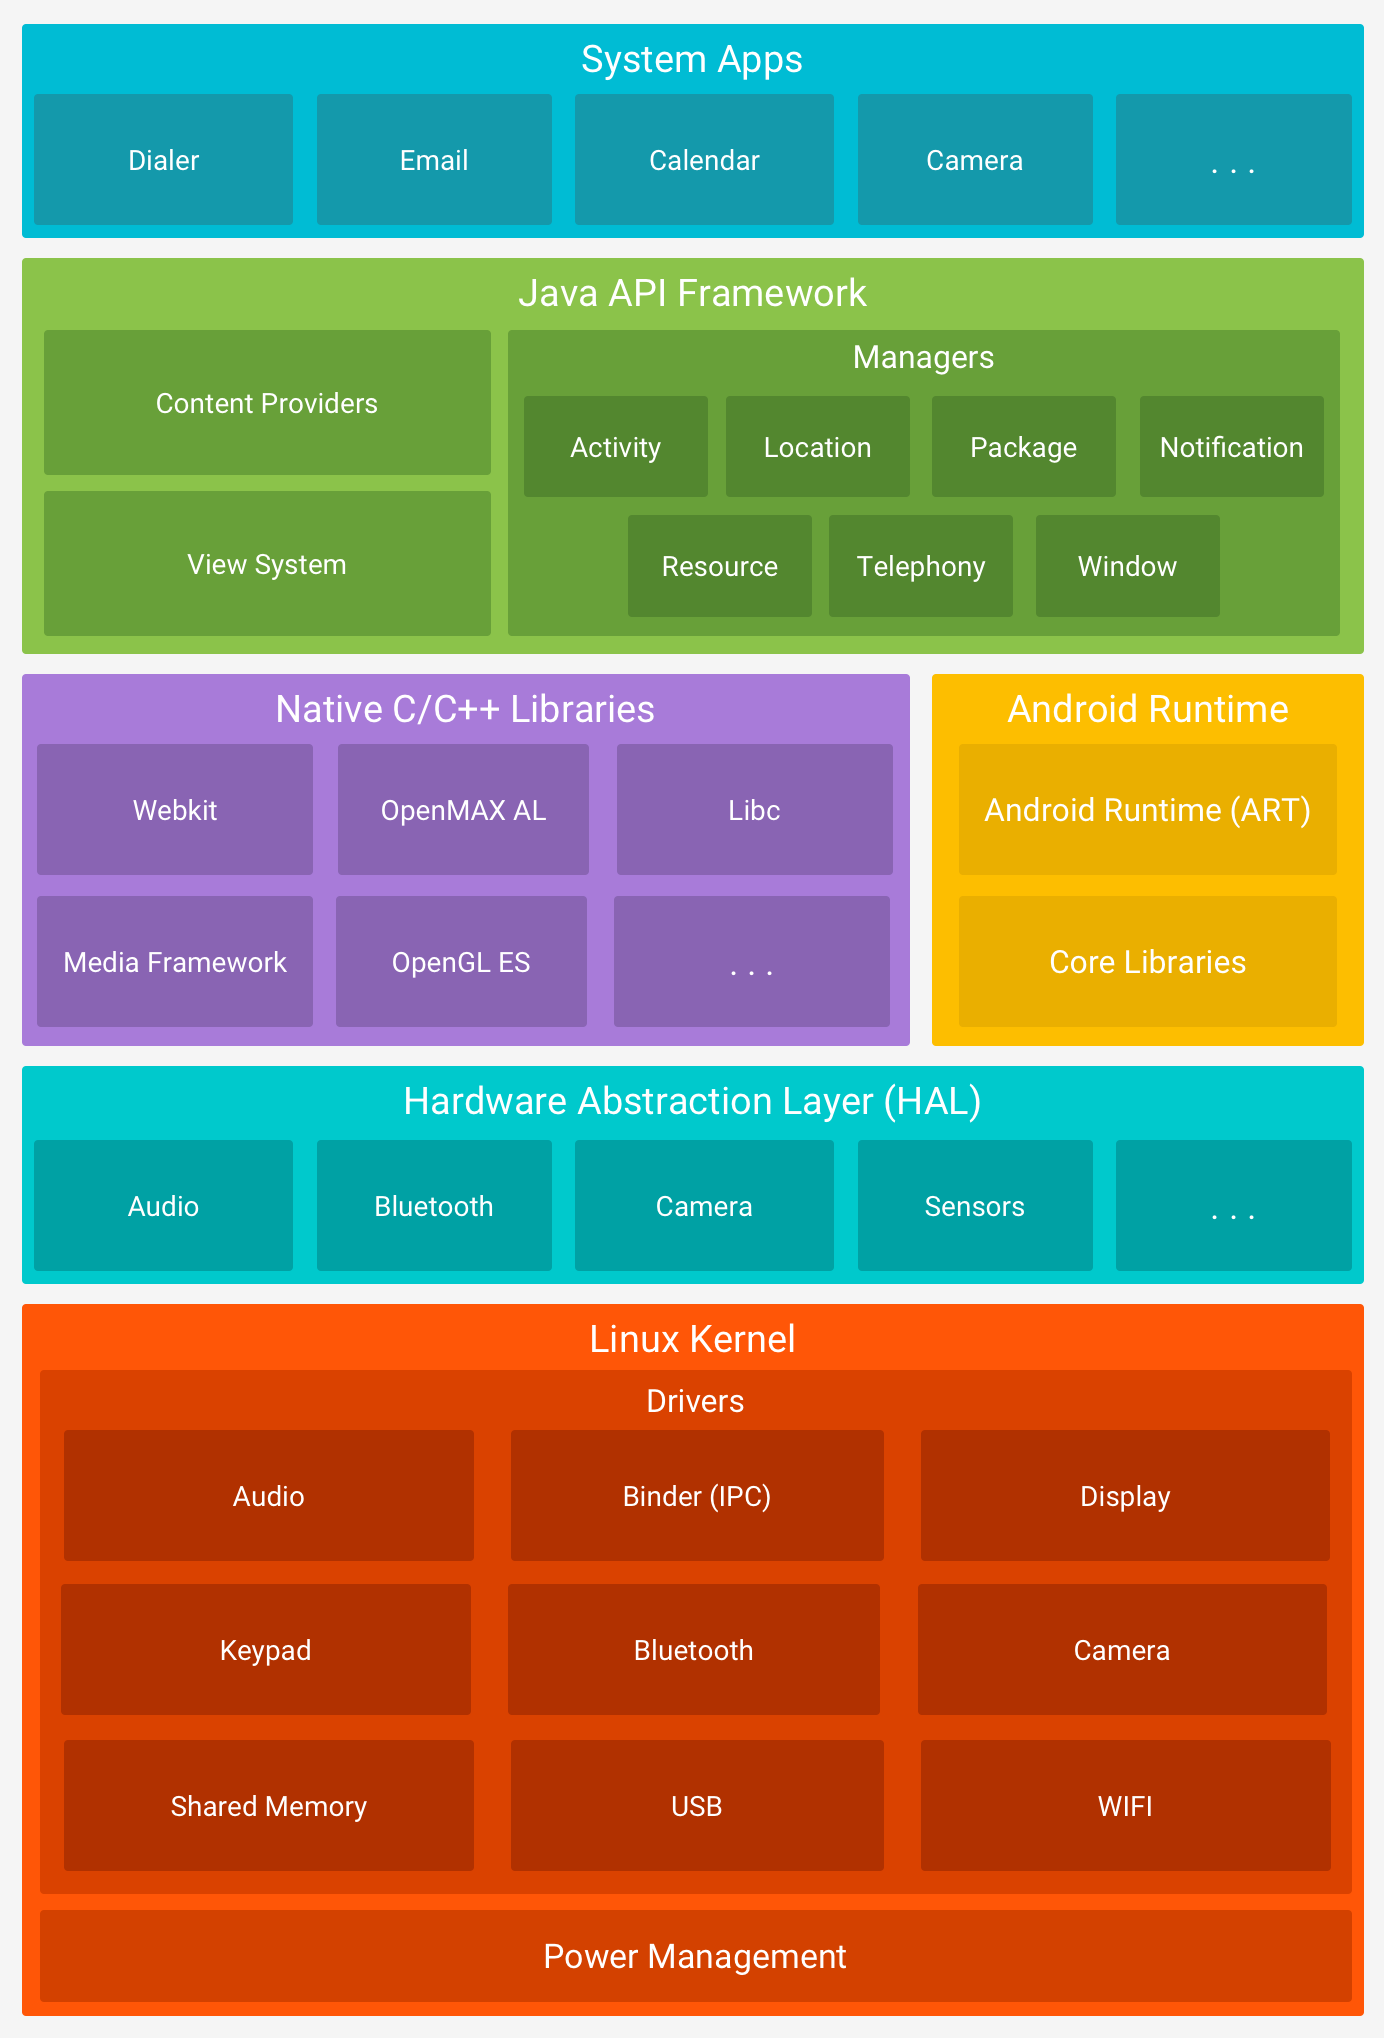
\includegraphics[width=0.68\linewidth]{figures/android_sw_stack-new.png}
      \end{figure}
    \end{columns}
\end{frame}

\begin{frame}{Android OS: Dalvik vs ART}
  \begin{figure}
    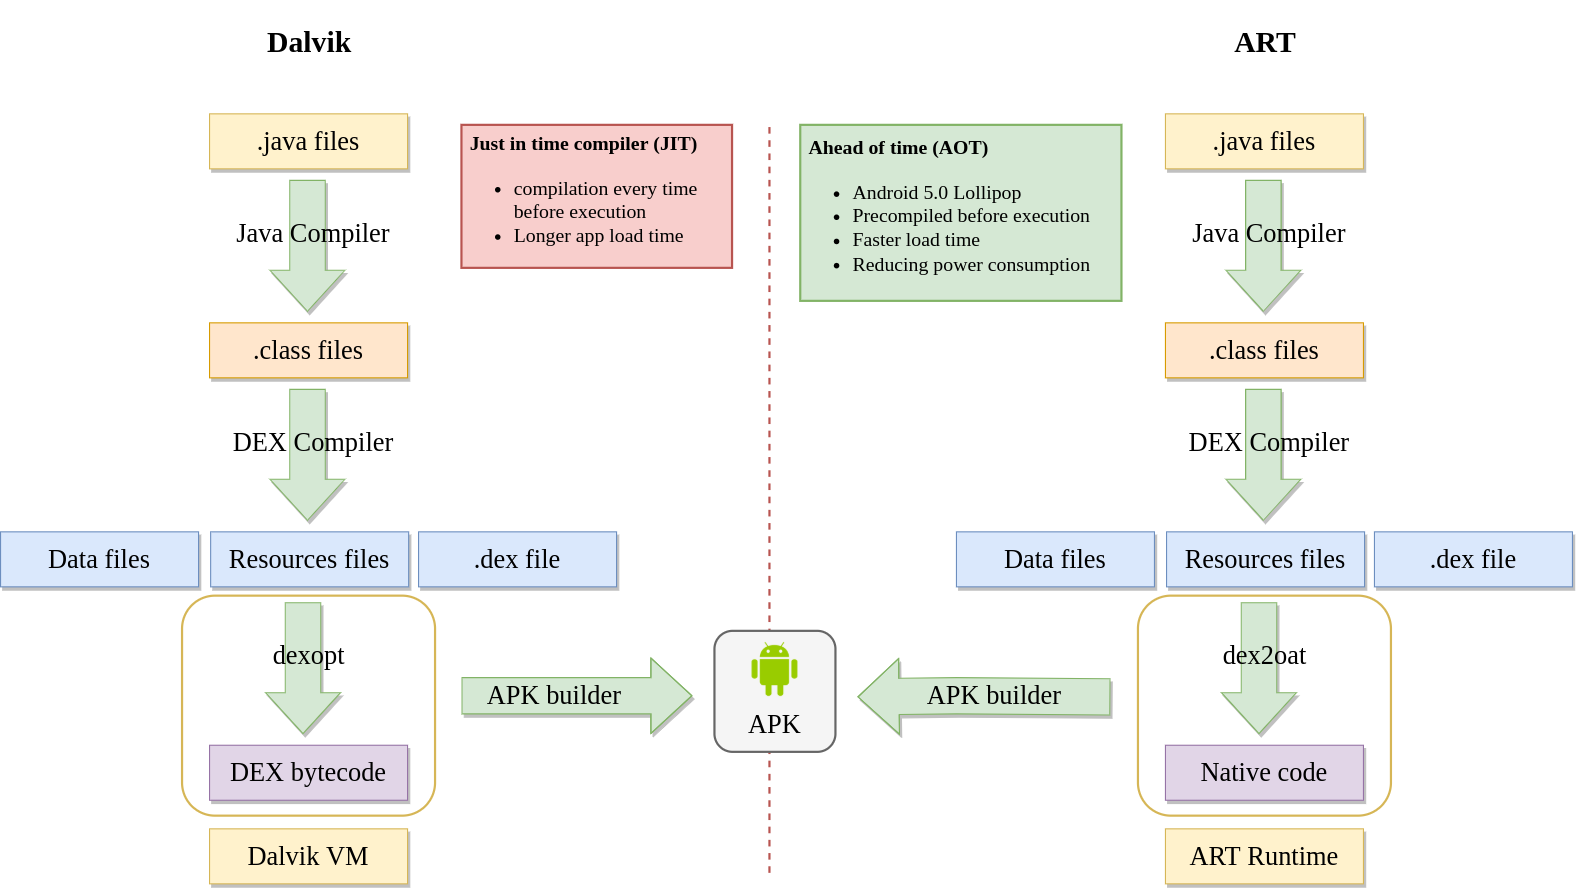
\includegraphics[width=1\linewidth]{figures/dalvik-vs-art.png}
  \end{figure}
\end{frame}

\section{Android Applications}

\begin{frame}{Android applications: Overview}
    \begin{block}{Languages}
      Applications are compiled using the SDK, the output is a \tcc{.apk} file.
      \begin{itemize}
        \item \tcc{Kotlin} in 2019 replaced Java and became the main language
        \item \tcc{Java} is still supported 
        \begin{itemize}
          \item some Java 8 functionalities require Android Studio (v. 3.0 or later).
        \end{itemize}
      \end{itemize}
    \end{block}
    \begin{block}{Device compatibility}
      Android can run on many different types of devices, it provides a dynamic app framework useful to
      define configuration-specific app resources:
      \begin{itemize}
        \item Device feature
        \item Platform version
        \item Screen configuration
      \end{itemize}
    \end{block}
\end{frame}

\subsection{Building Blocks}

\begin{frame}[allowframebreaks]{Android applications: Building Blocks}
  \begin{block}{Main Components}
    App components are the essential building blocks of an Android app:
    \begin{itemize}
      \item \tcc{Activity}
      \item \tcc{Service}
      \item \tcc{Content Provider}
      \item \tcc{Broadcast reciver}
    \end{itemize}
    Each type serves a distinct purpose and has a distinct lifecycle that defines how the \textit{component} is created and destroyed.
  \end{block}
  \newpage
  \begin{block}{1. Activity}
    \begin{itemize}
      \item An activity is the entry point for interacting with the user.
      \item It represents a screen with a UI defined using resource files (XML).
      \item The activities work together but each one is independent.
      \begin{itemize}
        \item  Ex. email app with many activities: editor, list, calendar.
      \end{itemize}
    \end{itemize}
  \end{block}

  \begin{block}{2. Service}
  \begin{itemize}
    \item It's a general-purpose entry point for keeping an app running in the background.
    \item It's not associated with a UI.
    \item Performs: long-running operations, work form remote processes.
    \begin{itemize}
      \item  Ex. play music in the background while the user is in a different app.
    \end{itemize}
  \end{itemize}
  \end{block}

  \begin{block}{3. Content Provider}
    \begin{itemize}
    \item It manages a shared set of data accessible from the app.
    \item The stored data can be private or shared with other applications.
    \end{itemize}
  \end{block}

  \begin{block}{4. Broadcast Receiver}
    \begin{itemize}
      \item It allows the app to respond to system-wide broadcast announcements
      \item The system can deliver broadcasts even to apps that aren't running
      \item Many broadcasts originate from the system:
      \begin{itemize}
        \item \textit{"battery is low"}, \textit{"the screen is turned off"} ...
      \end{itemize}
      \item It can activate a status bar notification:
      \begin{itemize}
        \item An app can schedule an alarm to post a notification.
      \end{itemize}
    \end{itemize}
  \end{block}
\end{frame}

\begin{frame}
  \frametitle{Building Blocks - Observations}
  \begin{enumerate}\itemsep20pt
    \item A unique aspect of Android system design is that any app can start another app’s component.
    \begin{itemize}
      \item Ex. If you want the user to capture a photo with the device camera, there's probably another app that does that. When complete, the photo is returned to your app.
    \end{itemize}
    \item Every components executes inside the app's control flow.
    \begin{itemize}
      \item Because the system runs each app in a separate process, your app cannot directly activate a component from another app. However, the Android system can.
    \end{itemize}
    \item Android apps don't have a single entry point (there's no \textit{main()} function).
  \end{enumerate}
\end{frame}

\subsection{The Manifest file}

\begin{frame}{The Manifest file}
\begin{columns}[c]
  \column{0.5\textwidth}
  \begin{itemize}\itemsep10pt
    \item Components shall be declared in the \tcc{AndroidManifest.xml}.
    \item The file must be located at the root of the app project directory.
    \item The manifest specifies a number of things:
    \begin{itemize}
      \item user permissions required.
      \item minimum API level.
      \item hardware and software features used by the app.
    \end{itemize}
  \end{itemize}
  \column{0.5\textwidth}
    \begin{exampleblock}{Example}
      \lstinputlisting[language=XML,basicstyle=\tiny]{./code/manifest.xml}
    \end{exampleblock}
  \end{columns}
\end{frame}

\subsection{Intent}

\begin{frame}{Activating components}
  \begin{block}{Intent}
    \begin{itemize}
      \item Components are activated by an asynchronous message called \tcc{Intent}.
      \begin{itemize}
        \item Unlike the others, \textit{Content Providers} are not activated by \textit{Intents}.
      \end{itemize}
      \item An \textit{Intent} defines the action to be executed and a set of additional information (\tcc{flag} and \tcc{extra}).
    \end{itemize}
  \end{block}
  \begin{block}{Intent types}
    \begin{itemize}
      \item \tcc{Explicit Intent}: created and invoked specifying the target app's package name.
      \begin{itemize}
        \item You'll typically start a component in your own app.
      \end{itemize}
      \item \tcc{Implicit Intent}: declare a general action to perform, the system will take care of it by finding the right component.
    \end{itemize}
  \end{block}
\end{frame}


\begin{frame}{Explict Intent: creation and usage}
  \begin{block}{How to build}
    You need instantiate a \tcc{android.content.Intent} class.
    \begin{itemize}
      \item It is considered a best practice to specify the \textit{Context} and the \textit{Class} of the component to instantiate:\newline\codeB{Intent(Context packageContext, Class<?> cls)}
      \item After creation, the system starts the component immediately.
    \end{itemize}
  \end{block}
  \begin{exampleblock}{Example}
    \lstinputlisting[language=Java]{./code/explicit-intent-example.java}
  \end{exampleblock}
\end{frame}

\begin{frame}[fragile,allowframebreaks]{Implict Intent: creation and usage}
  \begin{block}{How to build}
    Same as above, but the component is not specified:
    \begin{itemize}
      \item You must specify the action associated to the \textit{Intent} (\codeB{setAction()})
      \item You must check that there is a component capable of solving the \textit{Intent} (\codeB{resolveActivity()})
    \end{itemize}
  \end{block}
  \begin{exampleblock}{Example}
    \lstinputlisting[language=Java]{./code/implict-intent-example.java}
  \end{exampleblock}
  To define which implicit intents your app can receive, declare one or more intent filters
  for each of your app components with an \codeB{<intent-filter>} element in your manifest file.
  \begin{itemize}
    \item \tcc{<action>}: declares the intent action accepted;
    \item \tcc{<category>}: \textit{implicit intents} need \tcc{DEFAULT} category; 
    \item \tcc{<data>}: declares the type of data accepted;
  \end{itemize}
  \begin{exampleblock}{Example}
    \lstinputlisting[language=XML]{./code/intent-filter-example.xml}
  \end{exampleblock}
\end{frame}

\section*{References}
%-----------------------
%--- ONLINE RESURCES ---
%-----------------------

\begin{frame}{References - Online Resources}
\begin{thebibliography}{99}
\setbeamertemplate{bibliography item}[online]

\bibitem{adAPIguide} Android Developers - Guide
\newblock \link{https://developer.android.com/guide/}

\bibitem{adAPIreference} Android Developers - API Reference
\newblock \link{https://developer.android.com/reference/}

\bibitem{adTraining} Android Developers - Samples
\newblock \link{https://developer.android.com/samples/}

\bibitem{adTraining} Android Developers - Design \& Quality
\newblock \link{https://developer.android.com/design/}

\end{thebibliography}
\end{frame}

%-----------------------
%--- BOOKS -------------
%-----------------------

%\begin{frame}{Riferimenti - Libri}
%\begin{thebibliography}{99}
%\setbeamertemplate{bibliography item}[book]
%
%\bibitem{Mednieks11} Zigurd Mednieks, Laird Dornin, G. Blake Meike, Masumi Nakamura
%\newblock \emph{Programming Android}
%\newblock O'Reilly, 2011
%
%\bibitem{Haseman13} Chris Haseman, Kevin Grant
%\newblock \emph{Beginning Android Programming: Develop and Design}
%\newblock Peachpit Press, 2013
%
%\bibitem{Schwarz13} Ronan Schwarz, Phil Dutson, James Steele, Nelson To
%\newblock \emph{The Android Developer's Cookbook : Building Applications with the Android SDK}
%\newblock Addison-Wesley, 2013 
%
%\bibitem{Neil14} Theresa Neil
%\newblock \emph{Mobile Design Pattern Gallery: UI Patterns for Smartphone App}
%\newblock O'Relly, Second Edition, 2014
%\end{thebibliography}
%\end{frame}

\end{document}
